\section{Maintenance plan}


\subsection{DAG}

We define a maintenance plan as directed acyclic graph (DAG). We denote
the graph as $G=(V,G)$, where every vertex $v \in V$ corresponds to a 
base table or a materialized view and every edge $e \in E$ corresponds to a 
computation, e.g. $\sigma(A)$. The client operations flow from the origin of 
the graph, i.e. the base table, over the edges to the materialized views. The 
edge transforms the input stream into updates for subsequent views. Vertices 
without outgoing edges represent views that deliver the result to the client.

	
\textbf{Example --} 
Consider a client issuing the following query to the View Maintenance System:

\begin{verbatim}
	SELECT Sum(c2) FROM a GROUP BY c_1 WHERE c2 < 10
\end{verbatim} 

In the first naive approach the VMS translates every clause of the
query into a materialized view. The materialized views are concatenated
to build the final result of the query. The client can access the last
view to fetch the results. To 

\begin{figure}[h!] 
	\centering 
	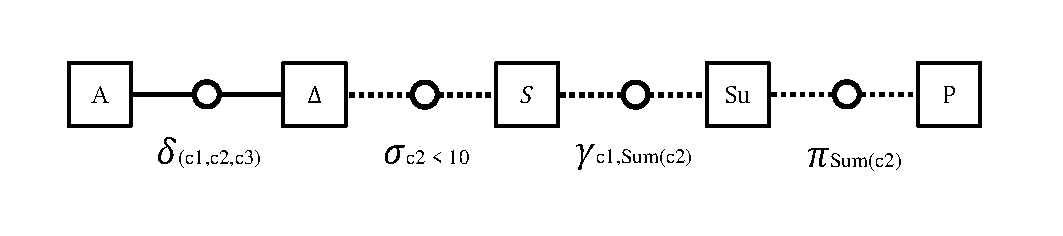
\includegraphics[width=\linewidth]{figures/MaintenanceExample}  
	\caption{Maintenance plan} 
	\label{fig:maintenance_plan} 
\end{figure} 

\subsection{Cost model}



\textbf{Cost model --} 
	Define node cost(storage)
	Define edge cost


\subsection{Optimization}

\textbf{Reorder operation --} 

	Algorithm reordering

\textbf{Merge operation --} 
	
	Algorithm reordering

The \textit{proceedings} are the records of a conference.
ACM, as well as PVLDB, seeks to give these conference by-products a uniform,
high-quality appearance.  To do this, ACM / PVLDB has some rigid
requirements for the format of the proceedings documents: there
is a specified format (balanced  double columns), a specified
set of fonts (Arial or Helvetica and Times Roman) in
certain specified sizes (for instance, 9 point for body copy),
a specified live area (18 $\times$ 23.5 cm [7" $\times$ 9.25"]) centered on
the page, specified size of margins (2.54cm [1"] top and
bottom and 1.9cm [.75"] left and right; specified column width
(8.45cm [3.33"]) and gutter size (.083cm [.33"]).

\subsection{SQL pattern}


The \textit{proceedings} are the records of a conference.
ACM, as well as PVLDB, seeks to give these conference by-products a uniform,
high-quality appearance.  To do this, ACM / PVLDB has some rigid
requirements for the format of the proceedings documents: there
is a specified format (balanced  double columns), a specified
set of fonts (Arial or Helvetica and Times Roman) in
certain specified sizes (for instance, 9 point for body copy),
a specified live area (18 $\times$ 23.5 cm [7" $\times$ 9.25"]) centered on
the page, specified size of margins (2.54cm [1"] top and
bottom and 1.9cm [.75"] left and right; specified column width
(8.45cm [3.33"]) and gutter size (.083cm [.33"]).


\begin{figure}[h!] 
	\centering 
	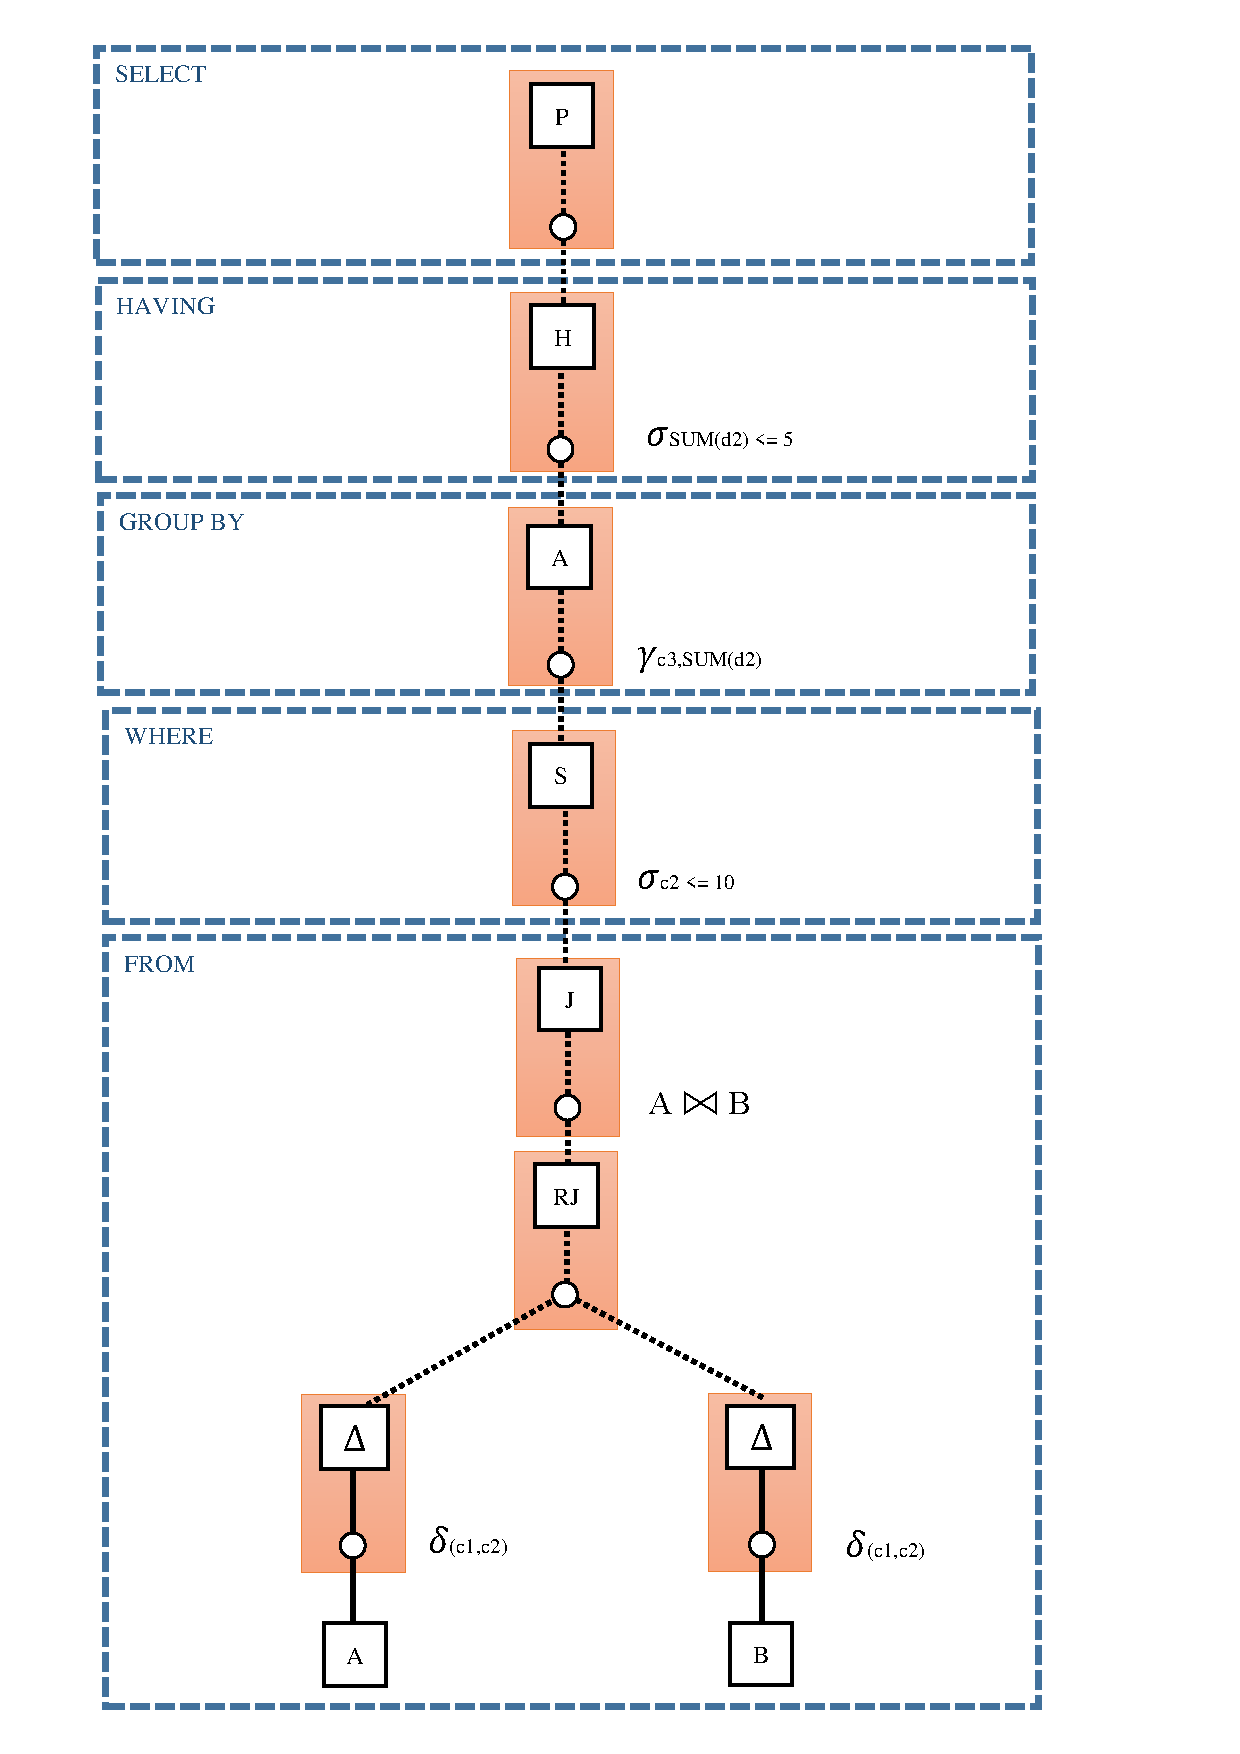
\includegraphics[width=\linewidth]{figures/SQLPattern}  
	\caption{SQL pattern} 
	\label{fig:sql_pattern} 
\end{figure} 

\subsection{Mapping}

	Clauses
	Evaluation order
	Mapping clauses -> view types



\subsection{Optimization}

Reorder
Merge 




The good news is, with only a handful of manual
settings\footnote{Two of these, the {\texttt{\char'134 numberofauthors}}
and {\texttt{\char'134 alignauthor}} commands, you have
already used; another, {\texttt{\char'134 balancecolumns}}, will
be used in your very last run of \LaTeX\ to ensure
balanced column heights on the last page.}, the \LaTeX\ document
class file handles all of this for you.

The remainder of this document is concerned with showing, in
the context of an ``actual'' document, the \LaTeX\ commands
specifically available for denoting the structure of a
proceedings paper, rather than with giving rigorous descriptions
or explanations of such commands.



